% ─────────────────────────────────────────────────────────────────────────────
%
% hardware_manager.tex
%
% Documentación del módulo hardware_manager:
%   - Comportamiento actual (UART → ESP32 → motores hápticos)
%   - Protocolo UART detallado
%   - Extensión para grabación de rosbag mediante GPIO en Raspberry Pi
%
% ─────────────────────────────────────────────────────────────────────────────

\section{Gestión de hardware y retroalimentación háptica}
\label{sec:hardware-manager}

El paquete \texttt{hardware\_manager} actúa como puente entre el ecosistema
ROS2 y el hardware de actuación háptica. Recibe mensajes de la capa de
percepción, los transforma en comandos de dutty cycle y los transmite a un
microcontrolador ESP32 a través de una interfaz UART serie. El ESP32, a su
vez, controla directamente los actuadores hápticos que proveen retroalimentación
vibrotáctil al usuario.

Esta separación entre el sistema de cómputo principal (Raspberry Pi) y el
microcontrolador dedicado (ESP32) responde a una decisión de arquitectura
deliberada: los tiempos de control de motores DC o actuadores de vibración
son más sensibles a la latencia que los algoritmos de percepción, y un
microcontrolador dedicado puede garantizar periodicidad de bucle sin
interferencia del sistema operativo de propósito general.

% ─────────────────────────────────────────────────────────────────────────────
\subsection{Nodo \texttt{grid\_to\_motor}}
\label{sec:hw-grid-to-motor}
% ─────────────────────────────────────────────────────────────────────────────

El ejecutable principal del paquete es \texttt{grid\_to\_motor}, implementado
en C++ como un nodo ROS2 heredado de \texttt{rclcpp::Node}. Sus
responsabilidades son:

\begin{enumerate}
  \item Suscribirse al tópico \texttt{/haptics/intensity\_grid} (mensaje
        \texttt{custom\_interfaces/msg/DepthGrid}).
  \item Convertir cada celda de la grilla de profundidad a un valor de
        \emph{duty cycle} en el rango $[0, 100]$.
  \item Serializar la grilla completa en una trama ASCII y transmitirla por
        UART.
\end{enumerate}

\subsubsection{Parámetros configurables}

\begin{table}[H]
\centering
\begin{tabular}{lll}
\toprule
\textbf{Parámetro} & \textbf{Valor por defecto} & \textbf{Descripción} \\
\midrule
\texttt{port}           & \texttt{/dev/ttyACM0} & Puerto serie \\
\texttt{baud}           & \texttt{115200}        & Velocidad en baudios \\
\texttt{topic}          & \texttt{/haptics/intensity\_grid}  & Tópico de entrada \\
\texttt{z\_min\_m}      & \texttt{0.25}          & Distancia mínima (m), duty = 100 \\
\texttt{z\_max\_m}      & \texttt{5.00}          & Distancia máxima (m), duty = 0   \\
\texttt{send\_period\_ms} & \texttt{50}          & Período mínimo entre envíos (ms) \\
\texttt{expected\_rows} & \texttt{5}             & Filas esperadas de la grilla \\
\texttt{expected\_cols} & \texttt{10}            & Columnas esperadas de la grilla \\
\texttt{duty\_scale}    & \texttt{0.4}           & Factor de escala del duty cycle \\
\bottomrule
\end{tabular}
\caption{Parámetros del nodo \texttt{grid\_to\_motor}.}
\label{tab:hw-params}
\end{table}

El factor de escala, no es mas que un ajuste de intensidad de vibracion evitando tener que
ajustarlo en el firmware de la ESP32 a la hora de hacer las pruebas.

\subsubsection{Conversión distancia → duty cycle}

La función de mapeo transforma la distancia medida $d$ (en metros) a un
duty cycle entero $D \in [0, 100]$ con la siguiente lógica:

\begin{equation}
  D(d) =
  \begin{cases}
    100 & \text{si } d \leq d_{\min} \\[4pt]
    0   & \text{si } d \geq d_{\max} \\[4pt]
    \displaystyle\left\lfloor
      \frac{d_{\max} - d}{d_{\max} - d_{\min}} \times 100 + 0{,}5
    \right\rfloor
    & \text{en otro caso}
  \end{cases}
\label{eq:duty}
\end{equation}

El valor resultante se escala adicionalmente por el factor
\texttt{duty\_scale} (por defecto $0{,}4$), lo que limita la vibración máxima
al $40\%$ del rango posible. Este parámetro permite ajustar la intensidad de
la retroalimentación sin modificar la lógica de mapeo de distancias.

\subsubsection{Throttling}

Para no saturar la interfaz UART, el nodo implementa un mecanismo de
throttling: sólo se transmite un nuevo frame si han transcurrido al menos
\texttt{send\_period\_ms} milisegundos desde el último envío. Este control
se realiza comparando marcas de tiempo de ROS2 (\texttt{rclcpp::Time}).

% ─────────────────────────────────────────────────────────────────────────────
\subsection{Enlace físico Raspberry Pi -- ESP32}
\label{sec:hw-enlace-fisico}
% ─────────────────────────────────────────────────────────────────────────────

La conexión entre la Raspberry Pi y la placa de desarrollo del ESP32 se
realiza mediante un único cable USB-A a USB-C de longitud reducida, que
cumple una doble función. En primer lugar, transporta los datos de control:
si bien el protocolo lógico es UART, cuya señalización es inherentemente
\emph{single-ended} (los niveles de TX y RX se referencian a un plano de
masa común), la transmisión física no ocurre directamente sobre esos pines.
La placa del ESP32 integra un puente USB-UART (\emph{USB-to-UART bridge}),
un circuito integrado dedicado que convierte las señales UART de nivel TTL
en tráfico USB. La cadena de comunicación resultante es:

\begin{center}
  nodo ROS2 $\xrightarrow{\texttt{/dev/ttyACM0}}$ pila USB del SO
  $\xrightarrow{\text{D+/D\textendash\ diferencial}}$ puente USB-UART
  $\xrightarrow{\text{UART TTL}}$ núcleo ESP32
\end{center}

El par D$+$/D$-$ emplea señalización diferencial: los bits se codifican como
la diferencia de tensión entre ambas líneas y no como un nivel absoluto
respecto a masa. Cualquier perturbación de modo común acoplada
simultáneamente en ambas líneas se cancela en el receptor, confiriéndole
una inmunidad al ruido electromagnético que la señalización UART directa no
posee de forma nativa. El blindaje del cable complementa esta protección
atenuando el acoplamiento con fuentes externas.

En segundo lugar, el cable alimenta el ESP32 a través de la línea VBUS
($5\,\mathrm{V}$) del puerto USB de la Raspberry Pi, eliminando la
necesidad de una fuente de alimentación independiente para el
microcontrolador.

% ─────────────────────────────────────────────────────────────────────────────
\subsection{Protocolo UART}
\label{sec:hw-uart-protocol}
% ─────────────────────────────────────────────────────────────────────────────

La comunicación entre la Raspberry Pi y el ESP32 utiliza UART con los
parámetros físicos descritos en la tabla~\ref{tab:uart-params}.

\begin{table}[H]
\centering
\begin{tabular}{ll}
\toprule
\textbf{Parámetro} & \textbf{Valor} \\
\midrule
Velocidad   & 115200 baudios \\
Bits de datos & 8 \\
Paridad       & Ninguna \\
Bits de parada & 1 \\
Control de flujo & Ninguno \\
Codificación & ASCII \\
\bottomrule
\end{tabular}
\caption{Parámetros físicos de la interfaz UART.}
\label{tab:uart-params}
\end{table}

\subsubsection{Formato de trama}

El protocolo utiliza tramas ASCII terminadas en newline
(\texttt{$\backslash$n}), lo que facilita enormemente la depuración
(basta un terminal serie para monitorear el tráfico) y la implementación del
receptor en el microcontrolador (lectura hasta \texttt{$\backslash$n}).

La trama es de tipo \textbf{M} (\emph{Motors}) y tiene el siguiente formato:

\begin{verbatim}
M <d0> <d1> ... <d49>\n
\end{verbatim}

donde:
\begin{itemize}
  \item \textbf{\texttt{M}} es el identificador de tipo de mensaje.
  \item \textbf{\texttt{d0}\ldots\texttt{d49}} son exactamente 50 enteros en
        el rango $[0, 100]$, cada uno representando el duty cycle del
        actuador correspondiente.
  \item El orden de los valores es \textbf{column-major de derecha a
        izquierda}: se recorren primero las columnas de la columna más a la
        derecha ($c = 9$) hacia la más a la izquierda ($c = 0$), y dentro
        de cada columna de arriba ($r = 0$) hacia abajo ($r = 4$). El índice
        resultante es
        $\text{idx} = (9 - c) \times 5 + r$,
        de modo que \texttt{d0} corresponde al motor en la esquina
        superior-derecha y \texttt{d49} al de la esquina inferior-izquierda
        (ambas vistas desde la perspectiva de la cámara).
  \item El separador entre campos es un espacio ASCII (\texttt{0x20}).
  \item La trama termina con \texttt{$\backslash$n} (\texttt{0x0A}).
\end{itemize}

\subsubsection{Disposición física de los motores}

La tabla~\ref{tab:motor-layout} muestra el índice $\text{d}_i$ de cada
motor en la matriz física de $5 \times 10$, tal como se ve desde la
perspectiva de la cámara (izquierda = lado izquierdo del usuario).

\begin{table}[H]
\centering
\begin{tabular}{c|cccccccccc}
\toprule
 & \textbf{c=9} & \textbf{c=8} & \textbf{c=7} & \textbf{c=6} & \textbf{c=5}
 & \textbf{c=4} & \textbf{c=3} & \textbf{c=2} & \textbf{c=1} & \textbf{c=0} \\
 & (der.) & & & & & & & & & (izq.) \\
\midrule
\textbf{r=0} & d0  & d5  & d10 & d15 & d20 & d25 & d30 & d35 & d40 & d45 \\
\textbf{r=1} & d1  & d6  & d11 & d16 & d21 & d26 & d31 & d36 & d41 & d46 \\
\textbf{r=2} & d2  & d7  & d12 & d17 & d22 & d27 & d32 & d37 & d42 & d47 \\
\textbf{r=3} & d3  & d8  & d13 & d18 & d23 & d28 & d33 & d38 & d43 & d48 \\
\textbf{r=4} & d4  & d9  & d14 & d19 & d24 & d29 & d34 & d39 & d44 & d49 \\
\bottomrule
\end{tabular}
\caption{Índice de cada motor en la trama UART. La esquina
  superior-derecha es \texttt{d0}; la inferior-izquierda es \texttt{d49}.}
\label{tab:motor-layout}
\end{table}

\subsubsection{Ejemplo de trama real (5×10)}

En la configuración nominal la trama contiene exactamente 50 valores y
tiene una longitud típica de unos 150--180 bytes:

\begin{verbatim}
M 40 38 35 30 20 40 38 35 28 18 35 33 30 25 15 30 28 25 20 10 ...
\end{verbatim}

\subsubsection{Decisiones de diseño del protocolo}

\textbf{ASCII en lugar de binario.}
Se eligió codificación ASCII por tres razones:
\begin{enumerate}
  \item \emph{Debuggabilidad}: cualquier terminal serie (p.\,ej.\
        \texttt{minicom}, \texttt{screen}, Arduino Serial Monitor) permite
        leer el tráfico directamente sin herramientas adicionales.
  \item \emph{Simplicidad de recepción}: el ESP32 puede acumular caracteres
        en un buffer y procesar la trama al recibir el newline, sin necesidad
        de gestionar longitudes de campo fijas ni checksums.
  \item \emph{Extensibilidad}: agregar nuevos tipos de mensaje se reduce a
        definir un nuevo identificador de tipo (un byte ASCII).
\end{enumerate}

Una alternativa más compacta consiste en representar cada valor en binario
puro, aprovechando que el rango $[0, 100]$ cabe en $\lceil \log_2 101 \rceil = 7$
bits. Empaquetando los 50 valores sin padding, la trama quedaría en
$\lceil 50 \times 7 / 8 \rceil = 44$ bytes de carga útil más un byte de
cabecera, totalizando 45~bytes. Comparando los tiempos de transmisión a
115200~baudios con codificación 8N1 (10~bits por byte incluyendo bits de
inicio y parada):

\begin{align}
  t_{\mathrm{ASCII}}  &= \frac{160 \times 10}{115200} \approx 13{,}9\,\mathrm{ms} \\[4pt]
  t_{\mathrm{binario}} &= \frac{45 \times 10}{115200}  \approx  3{,}9\,\mathrm{ms}
\end{align}

Ambos valores son sustancialmente menores que el período mínimo de envío
de 50~ms configurado en el nodo (parámetro \texttt{send\_period\_ms}), por
lo que la diferencia de $\approx 10\,\mathrm{ms}$ no tiene impacto práctico
en la latencia del sistema. Esto refuerza la elección de ASCII: la penalización
en ancho de banda es despreciable frente a las ventajas de depuración y
simplicidad de implementación.

\textbf{Identificador de tipo al comienzo.}
El primer campo \texttt{M} permite al receptor descartar tramas parciales o
corruptas de forma sencilla: si el primer byte no corresponde a un identificador
reconocido, la trama se descarta.

Adicionalmente, este campo fue concebido como punto de extensión para futuros
mensajes de configuración. Por ejemplo, podrían enviarse tramas iniciadas con
el carácter \texttt{`C'} para transmitir parámetros al microcontrolador sin
requerir cambios en el protocolo. Dicha funcionalidad no fue implementada al
no resultar necesaria durante el desarrollo, aunque su incorporación requeriría
únicamente extender la lógica de \emph{parsing} en el firmware del ESP32.

\textbf{Longitud fija implícita.}
La trama contiene siempre exactamente 50 valores, lo que simplifica la
implementación del receptor: basta esperar 50 enteros separados por espacios
tras el identificador \texttt{M}, sin necesidad de leer dimensiones
dinámicas.

\textbf{Ausencia de checksum.}
No se implementó un mecanismo de verificación de integridad (\emph{checksum}).
Dos factores hacen que dicha omisión sea justificada. Por un lado, las
condiciones del enlace físico son favorables: como se describe en la
sección~\ref{sec:hw-enlace-fisico}, la señalización diferencial USB y la
baja velocidad de transmisión (115200~bps) resultan en una tasa de error de
bit despreciable. Por otro lado, el impacto de una trama corrupta es
bajo: los valores de \emph{duty cycle} se actualizan de forma continua al
ritmo del período de envío (texttt{send\_period\_ms}), por lo que un
fotograma incorrecto produce, a lo sumo, una perturbación vibrotáctil
puntual que la trama siguiente corrige de forma inmediata.

\subsubsection{Comportamiento en el ESP32}

El firmware del ESP32 debe implementar la siguiente lógica de recepción:

\begin{enumerate}
  \item Leer bytes del UART hasta encontrar \texttt{$\backslash$n}.
  \item Parsear el primer token. Si es \texttt{'M'}, procesar como trama
        de motores; de lo contrario, descartar.
  \item Leer los 50 valores de duty cycle.
  \item Aplicar los valores a los PWM de los actuadores según el índice
        $\text{idx} = (9 - c) \times 5 + r$ (column-major, de derecha a
        izquierda).
\end{enumerate}

Un timeout de recepción es recomendable: si no se recibe ninguna trama en
más de $\sim$500\,ms, el ESP32 debería poner todos los actuadores en duty
$= 0$ como medida de seguridad.

% ─────────────────────────────────────────────────────────────────────────────
\subsection{Nodo auxiliar: \texttt{motor\_sweep\_uart}}
\label{sec:hw-motor-sweep}
% ─────────────────────────────────────────────────────────────────────────────

El paquete incluye un segundo ejecutable, \texttt{motor\_sweep\_uart}, destinado
a pruebas de calibración y diagnóstico. Este nodo no suscribe ningún tópico
ROS2; en cambio, genera una secuencia periódica de duty cycles predefinida
$\{0, 25, 50, 75, 100\}$ y la transmite por UART para verificar que los
actuadores respondan correctamente a todo el rango de valores.

% ─────────────────────────────────────────────────────────────────────────────
\section{Grabación de rosbag mediante control GPIO}
\label{sec:gpio-rosbag-controller}
% ─────────────────────────────────────────────────────────────────────────────

\subsection{Problema y motivación}
\label{sec:gpio-rosbag-motivation}

Durante experimentos de campo el sistema opera de forma completamente autónoma:
la Raspberry Pi arranca a partir de una batería portátil, lanza el stack de
percepción y actúa sin supervisión de una computadora externa. En este escenario
surge la necesidad de controlar la grabación de datos (\emph{rosbag}) sin
disponer de teclado, ratón ni conexión de red.

Los requerimientos concretos son:
\begin{itemize}
  \item Iniciar y detener la grabación con un interruptor físico.
  \item Obtener retroalimentación visual inmediata sobre el estado del sistema
        mediante un LED.
  \item Garantizar que las bolsas de datos no queden corruptas ante una
        detención abrupta.
  \item Sobrevivir a fallos del proceso de grabación sin reiniciar el stack
        de percepción.
\end{itemize}

\subsection{Solución propuesta: \texttt{gpio\_rosbag\_controller}}
\label{sec:gpio-rosbag-solution}

Se diseñó el paquete ROS2 \texttt{gpio\_rosbag\_controller}, un nodo C++ de
bajo peso que se ejecuta en paralelo al stack de percepción y gestiona
exclusivamente el ciclo de vida de la grabación.

\subsubsection{Semántica del interruptor}

\begin{table}[H]
\centering
\begin{tabular}{lll}
\toprule
\textbf{Transición} & \textbf{Acción} & \textbf{LED} \\
\midrule
$0 \to 1$ (encendido) & Iniciar \texttt{ros2 bag record}   & SÓLIDO durante inicio; PARPADEO al confirmar \\
$1 \to 0$ (apagado)   & Enviar SIGINT al proceso de grabación & SÓLIDO durante cierre; APAGADO al terminar \\
\bottomrule
\end{tabular}
\caption{Semántica de las transiciones del interruptor físico.}
\label{tab:switch-semantics}
\end{table}

\subsubsection{Semántica del LED}

\begin{table}[H]
\centering
\begin{tabular}{ll}
\toprule
\textbf{Estado LED}  & \textbf{Significado} \\
\midrule
APAGADO  & Inactivo — no se está grabando \\
SÓLIDO   & Transición (iniciando o deteniendo grabación) \\
PARPADEO & Grabación activa \\
\bottomrule
\end{tabular}
\caption{Semántica visual del LED de estado.}
\label{tab:led-semantics}
\end{table}

\subsubsection{Máquina de estados}

El nodo implementa una máquina de estados con cuatro estados:

\begin{enumerate}
  \item \textbf{IDLE}: sistema inactivo, LED apagado.
  \item \textbf{STARTING}: interruptor activado, proceso de grabación en
        lanzamiento, LED sólido.
  \item \textbf{RECORDING}: grabación activa confirmada, LED parpadeando.
  \item \textbf{STOPPING}: interruptor desactivado, esperando cierre limpio
        del proceso, LED sólido.
\end{enumerate}

Las transiciones son:
\begin{align*}
  \text{IDLE}      &\xrightarrow{\text{switch}=1} \text{STARTING} \\
  \text{STARTING}  &\xrightarrow{\text{bag vivo (watchdog)}} \text{RECORDING} \\
  \text{RECORDING} &\xrightarrow{\text{switch}=0} \text{STOPPING} \\
  \text{STOPPING}  &\xrightarrow{\text{bag terminado}} \text{IDLE} \\
  \text{RECORDING} &\xrightarrow{\text{crash inesperado}} \text{IDLE}
\end{align*}

Todas las transiciones son accionadas por \emph{timers} de ROS2; no existe
ningún bucle bloqueante.

\subsubsection{Decisión de arquitectura: subprocess vs.\ API \texttt{rosbag2\_cpp}}

Se evaluaron dos enfoques para controlar la grabación:

\begin{table}[H]
\centering
\begin{tabular}{lll}
\toprule
\textbf{Criterio} & \textbf{subprocess} & \textbf{API rosbag2\_cpp} \\
\midrule
Aislamiento de fallos & Proceso separado & Mismo proceso \\
Cierre limpio          & SIGINT → flush    & Requiere gestión manual \\
Complejidad            & Baja              & Alta \\
Recuperación ante crash & Controlador sobrevive & Ambos fallan \\
\bottomrule
\end{tabular}
\caption{Comparación de enfoques para control de rosbag.}
\label{tab:rosbag-approaches}
\end{table}

Se eligió el enfoque de \emph{subprocess}: al lanzar \texttt{ros2 bag record}
como un proceso hijo independiente, el nodo controlador sobrevive a cualquier
fallo del proceso de grabación, y el cierre limpio se garantiza enviando
SIGINT al grupo de procesos y esperando la terminación mediante
\texttt{waitpid()}.

% ─────────────────────────────────────────────────────────────────────────────
\subsection{Conexionado GPIO}
\label{sec:gpio-wiring}
% ─────────────────────────────────────────────────────────────────────────────

\subsubsection{Asignación de pines}

\begin{table}[H]
\centering
\begin{tabular}{lllll}
\toprule
\textbf{Señal} & \textbf{Dirección} & \textbf{GPIO BCM} & \textbf{Pin físico} & \textbf{Notas} \\
\midrule
Interruptor & Entrada & BCM 17 & Pin 11 & Pull-down externo $10\,\mathrm{k}\Omega$ \\
LED         & Salida  & BCM 27 & Pin 13 & Resistencia serie $330\,\Omega$         \\
\bottomrule
\end{tabular}
\caption{Mapa de pines GPIO para el controlador de grabación.}
\label{tab:gpio-map}
\end{table}

Los números BCM son configurables a través del archivo de parámetros
\texttt{params.yaml} sin necesidad de recompilar el nodo.

\begin{figure}[H]
\centering
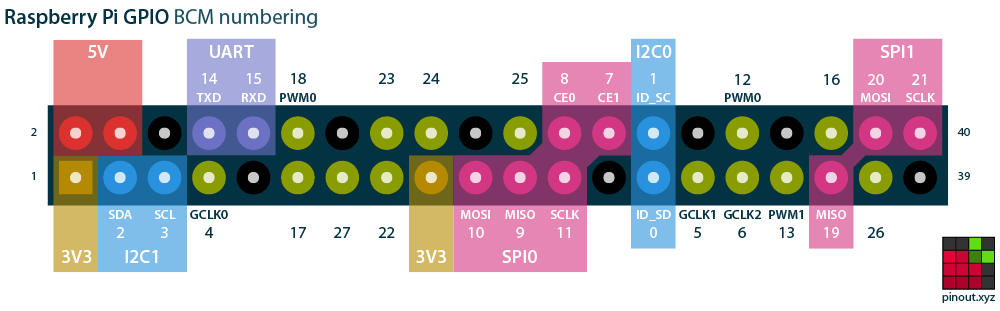
\includegraphics[width=\linewidth]{Notas/img/rpi-pinout.png}
\caption{Pinout del conector GPIO de 40 pines de la Raspberry Pi.
  Los pines utilizados son: \textbf{Pin~1} (3{,}3\,V, VCC del
  interruptor), \textbf{Pin~6} (GND, pull-down del interruptor),
  \textbf{Pin~9} (GND, cátodo del LED), \textbf{Pin~11} (BCM17, entrada
  del interruptor) y \textbf{Pin~13} (BCM27, salida hacia el LED).
  Imagen: \url{https://pinout.xyz}.}
\label{fig:rpi-pinout}
\end{figure}

\subsubsection{Conexión del interruptor}

El interruptor conecta la línea BCM 17 a la tensión de $3{,}3\,\mathrm{V}$.
Una resistencia de pull-down de $10\,\mathrm{k}\Omega$ mantiene la línea en
nivel lógico bajo cuando el interruptor está abierto, evitando lecturas
flotantes que podrían generar transiciones espurias.

\begin{figure}[H]
\centering
\begin{verbatim}
  3.3V (Pin 1) ----[ INTERRUPTOR ]---- BCM 17 (Pin 11)
                                              |
                                           10 kOhm
                                              |
                                           GND (Pin 6)
\end{verbatim}
\caption{Diagrama de conexión del interruptor físico.}
\label{fig:switch-wiring}
\end{figure}

\subsubsection{Conexión del LED}

El LED se conecta en serie con una resistencia de $330\,\Omega$ entre la
salida GPIO BCM 27 y masa.

La resistencia se calcula a partir de la tensión de alimentación
$V_{cc} = 3{,}3\,\mathrm{V}$, la tensión directa del LED
$V_f \approx 2{,}0\,\mathrm{V}$ y una corriente de diseño
$I_f = 10\,\mathrm{mA}$:

\begin{equation}
  R = \frac{V_{cc} - V_f}{I_f} = \frac{3{,}3 - 2{,}0}{0{,}010} = 130\,\Omega
\end{equation}

El valor comercial de $330\,\Omega$ proporciona
$I_f \approx 4\,\mathrm{mA}$, perfectamente visible en exteriores y dentro
del límite de $16\,\mathrm{mA}$ por pin de la Raspberry Pi.

\begin{figure}[H]
\centering
\begin{verbatim}
  BCM 27 (Pin 13) --[ 330 Ohm ]--[>|-- GND (Pin 9)
                                 LED
\end{verbatim}
\caption{Diagrama de conexión del LED de estado.}
\label{fig:led-wiring}
\end{figure}

\subsubsection{Consideraciones eléctricas}

\begin{itemize}
  \item Los pines GPIO de la Raspberry Pi operan a $3{,}3\,\mathrm{V}$
        y \textbf{no son tolerantes a $5\,\mathrm{V}$}. Cualquier señal
        externa que supere $3{,}3\,\mathrm{V}$ en un pin GPIO dañará
        permanentemente el SoC.
  \item La corriente máxima por pin es $16\,\mathrm{mA}$; la corriente
        total de todos los GPIOs simultáneamente no debe superar
        $50\,\mathrm{mA}$.
  \item Para cargas inductivas (relés, motores) se requieren diodos de
        protección; este diseño no las incluye.
\end{itemize}

% ─────────────────────────────────────────────────────────────────────────────
\subsection{Tópicos grabados}
\label{sec:gpio-rosbag-topics}
% ─────────────────────────────────────────────────────────────────────────────

Se graban únicamente los tópicos necesarios para análisis \emph{offline} de
odometría visual-inercial y profundidad. Los metadatos de la cámara y
\texttt{/parameter\_events} se excluyen por defecto.

\begin{table}[H]
\centering
\begin{tabular}{ll}
\toprule
\textbf{Tópico} & \textbf{Justificación} \\
\midrule
\texttt{.../aligned\_depth\_to\_color/image\_raw}  & Profundidad alineada al color \\
\texttt{.../aligned\_depth\_to\_color/camera\_info}& Parámetros intrínsecos \\
\texttt{.../color/image\_raw}                      & Imagen RGB \\
\texttt{.../color/camera\_info}                    & Parámetros intrínsecos color \\
\texttt{.../accel/sample}                          & Acelerómetro IMU \\
\texttt{.../gyro/sample}                           & Giróscopo IMU \\
\texttt{.../imu}                                   & IMU combinado \\
\texttt{.../accel/imu\_info}                       & Calibración acelerómetro \\
\texttt{.../gyro/imu\_info}                        & Calibración giróscopo \\
\texttt{.../extrinsics/depth\_to\_color}           & Transformación extrínseca \\
\texttt{.../extrinsics/depth\_to\_accel}           & Transformación extrínseca \\
\texttt{.../extrinsics/depth\_to\_gyro}            & Transformación extrínseca \\
\texttt{/tf\_static}                               & Árbol de transformadas fijas \\
\texttt{/rosout}                                   & Logs del sistema \\
\bottomrule
\end{tabular}
\caption{Tópicos grabados por defecto.}
\label{tab:rosbag-topics}
\end{table}

% ─────────────────────────────────────────────────────────────────────────────
\subsection{Integración con systemd}
\label{sec:gpio-systemd}
% ─────────────────────────────────────────────────────────────────────────────

El controlador se registra como servicio \texttt{systemd} para iniciar
automáticamente con el sistema operativo. El servicio configura el entorno
de ROS2 mediante una línea \texttt{ExecStart} que sourcea los archivos de
setup del workspace antes de lanzar el nodo:

\begin{verbatim}
ExecStart=/bin/bash -c '
  source /opt/ros/humble/setup.bash &&
  source /home/pi/nav_mapper/install/setup.bash &&
  exec ros2 launch gpio_rosbag_controller
       gpio_rosbag_controller.launch.py'
\end{verbatim}

La política \texttt{Restart=on-failure} con \texttt{RestartSec=5s}
garantiza que el controlador se relance automáticamente si falla por
cualquier razón externa (por ejemplo, un error transitorio de GPIO al
arranque).
